\documentclass{beamer}

\usepackage[utf8]{inputenc}
\usepackage[russian]{babel}
\usepackage{amsmath}
\usepackage{beamerthemesplit}
\usetheme[numbers, totalnumbers, compress, nologo]{Statmod}

\title{Алгоритмы и реализация решения задачи сборки ДНК из paired-end данных для сверхбольших геномов}
\author{Владислав Исенбаев}
\institute[СПбНИУ ИТМО]{Санкт-Петербургский национальный исследовательский\\
университет информационных технологий, механики \\
и оптики\\
\vspace{0.4cm}
Научный руководитель: д.т.н., проф. Шалыто~А.~А.}
\date{Санкт-Петербург\\2012 г.}

\begin{document}

\frame{\titlepage}

\section[Содержание]{}
\frame{\tableofcontents}

\section{Исходная задача}
\subsection{Высокопроизводительное секвенирование ДНК}
\frame {
  \frametitle{ДНК}
  Дезоксирибонуклеиновая кислота (ДНК).
  
  \begin{itemize}
  \item<1-> Двойная спираль из двух полимерных цепочек.
  \item<2-> Составные элементы~--- нуклеотиды.
  \item<3-> Комплементарность (A-T, G-C).
  \end{itemize}
}
\frame {
  \frametitle{Метод секвенирования double-ended shotgun} 

  \begin{itemize}
  \item<1-> Амплификация исходной ДНК.
  \item<2-> Разрезание ДНК на фрагменты.
  \item<3-> Выделение фрагментов подходящей длины ($ins=~250$ оснований).
  \item<4-> Чтение префикса и суффикса каждого фрагмента (по $n=36$ оснований каждый).
  \item<5-> Обработка полученных данных.
  \end{itemize}

%  \begin{figure}
%    \center{
%      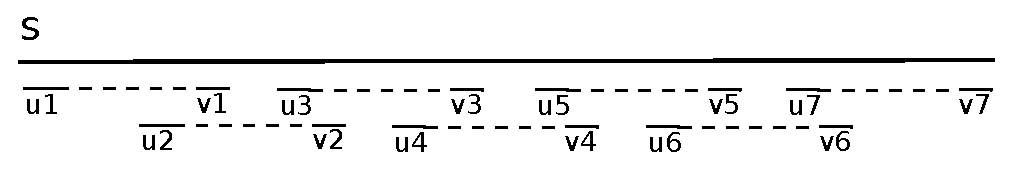
\includegraphics[width=100mm]{../pic/general.svg.eps}
%    }
  \end{figure}
}
%\frame {
%  \frametitle{Проблемы}
%  
%  \begin{itemize}
%  \item<1-> Большой объем данных.
%  \item<2-> Ошибки чтения.
%  \item<3-> Полиморфизм.
%  \end{itemize}
%}
%\section{Существующие методы решения задачи}
%\frame{
%  \frametitle{Схема решения}
%  \begin{itemize}
%  \item<1-> Фильтрация ошибок.
%  \item<2-> Решение задачи без использования paired-end данных.
%  \item<3-> Синтез полученных контигов в более длинные последовательности опираясь на paired-end данные.
%  \end{itemize}
%}
\section{Предлагаемое решение}
\frame{
  \frametitle{Схема решения}
  
  \begin{itemize}
  \item<1-> Фильтрация ошибок.
  \item<2-> Построение сжатого графа де Брейна.
  \item<3-> Удаление ошибочных ветвлений, используя paired-end данные.
  \item<4-> Схлоп полиморфных последовательностей.
  \item<5-> Раскрутка циклов с использованием paired-end данных.
  \end{itemize}
}
\frame{
  \frametitle{Алгоритм восстановления фрагментов}
  Построим по исходным данным сжатый граф де Брейна с
  последовательностями в вершинах длиной $k$ .

%  \begin{figure}
%    \center{
%      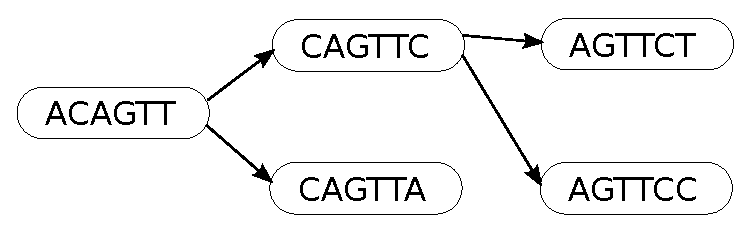
\includegraphics[width=100mm]{../pic/debrujin.svg.eps}
%    }
  \end{figure}

  Найдем места в графе, соответствующие началу и концу
  фрагмента. Тогда полным прочтениям фрагмента будут
  соответствовать пути из начального в конечное положение длиной $ins-k$.
}
\frame{
  \frametitle{Оптимизации}
  
  \begin{itemize}
  \item<1-> Отсечение по расстоянию до конечной вершины.
  \item<2-> Динамическое программирование.
  \end{itemize}
}
\frame{
  \frametitle{Использование алгоритма восстановления фрагментов}
  
  \begin{itemize}
  \item<1->Устранение ошибочных ветвлений и разъединение слипшихся путей.
  \item<2->Разворачивание циклов.
  \end{itemize}
}
\section{Результаты}
\frame {
  \frametitle{Escherichia Coli}
  
  \begin{itemize}
    \item<1-> Покрытие генома контигами: $95\%$
    \item<2-> Количество контигов длиннее $100$ оснований: $2800$
    \item<2-> Самый длинный контиг: $35419$ оснований
    \item<3-> $N50=6375$
  \end{itemize}
}
\frame {
  \frametitle{Спасибо за внимание!}
  Вопросы?
}
\end{document}
